\documentclass{beamer}
\usepackage{listings}
\lstset{
%language=C,
frame=single, 
breaklines=true,
columns=fullflexible
}

\usepackage{subcaption}
\usepackage{url}
\setbeamertemplate{caption}[numbered]
\usepackage{tikz}
\usepackage{pgfplots}
\pgfplotsset{compat=1.17}
\usepackage{tkz-fct}
\usepackage{mathrsfs}
\usepackage{txfonts}
\usepackage{tkz-euclide} 
\usetikzlibrary{calc,math}
\usepackage{float}
\newcommand\norm[1]{\left\lVert#1\right\rVert}
\renewcommand{\vec}[1]{\mathbf{#1}}
\providecommand{\pr}[1]{\ensuremath{\Pr\left(#1\right)}}
\usepackage[export]{adjustbox}
\usepackage[utf8]{inputenc}
\usepackage{amsmath}
\usetheme{Boadilla}
\title{Optimal LAP Altitude for Maximum Coverage}
\author{Chitneedi Geetha Sowmya - CS20BTECH11011}

\begin{document}

\begin{frame}
\titlepage
\end{frame}


% \begin{frame}{Outline}

% \begin{enumerate}
%     \item Introduction and motivation
%     \item Preliminaries required for radio propagation model
%     \item Modeling Line of Sight Probability
%     \item Methodology for obtaining the optimum LAP altitude
%     \item Finding the optimal LAP altitude
% \end{enumerate}

% \end{frame}

\section{Introduction and Motivation}

\begin{frame}{Introduction}
\begin{enumerate}
    \item Broadband wireless networks are increasingly adopted by users of mission critical communications, such as public safety agencies and first responders.
    \item Like every cellular network, the communication is largely dependent on fixed infrastructure (base stations) that could be severally disrupted in the case of natural disasters such as floods, earthquakes or tsunamis.
    \item One of the temporary recovery solution which is rapid and cost-effective for realizing wireless recovery networks is by utilizing airborne base stations.
    \item Airborne network recovery solutions mainly focuses on Low Altitude Platforms (LAPs).
\end{enumerate}
\end{frame}


\begin{frame}{LAP}

\begin{block}{What is LAP ?}
\begin{enumerate}
    \item Low Altitude Platform (LAP) is a quasi-stationary aerial platform usually characterized with an altitude laying within the troposphere.
    \item It is used as an alternative solution to emergency communication system.
    \item Examples: quad-copters, balloons and helicopter.
\end{enumerate}
\end{block}

\begin{block}{Why LAP ?}
\begin{enumerate}
    \item LAPs are much easier to deploy, and are inline with the broadband cellular concept.
    \item Low altitude combines both coverage superiority and confined cell radius.
\end{enumerate}
\end{block}

\end{frame}

\begin{frame}{Motivation}

\begin{enumerate}
    \item Due to technical limitations, the number of deployable LAPs could be very limited.
    \item So in order to provide the best possible coverage,we need  full exploitation of each of the deployed LAPs by optimizing its altitude.
    \item Let’s discuss about a mathematical model capable of predicting the optimum altitude of a LAP based on the statistical parameters of the underlying urban environment.
\end{enumerate}

\end{frame}


\section{Preliminaries required for radio propagation model }
\begin{frame}{Preliminaries required for radio propagation model}
        \begin{block}{Classification of propagation groups}
     Air-To-Ground (ATG) communication occurs in accordance to two main propagation groups. where,
    \begin{enumerate}
        \item First group : Receivers favoring a Line-of-Sight (LoS) condition or near-Line-of-Sight condition.
        \item Second group: Receivers with no LAP Line-of-Sight but still receiving coverage via strong reflections and diffractions.
    \end{enumerate}

        \end{block}
    
    \begin{block}{What is Line of sight(LoS)?}
A straight line between a transmitting antenna and receiving antenna when unobstructed by horizon.
\end{block}
    
\end{frame}

\begin{frame}{Low Altitude Platforms radio propagation in urban environment }

\begin{figure}
    \centering
    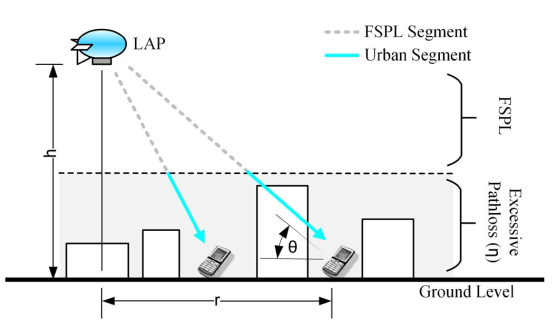
\includegraphics[width=10cm, height=4cm]{Figures/Figure1.png}
    \caption{Low Altitude Platforms radio propagation in urban environment}
    \label{fig:1}
\end{figure}
Radio signals emitted by a LAP base station propagate in free space until reaching the urban environment where they incur shadowing and scattering caused by the man-made structures, creating an additional loss in the ATG link.

\end{frame}

\begin{frame}{Let's understand some terms}
    \begin{block}{PL}
    PathLoss is the reduction in power density (attenuation) of an electromagnetic wave as it propagates through space
    \end{block}
    
     \begin{block}{FSPL}
   Free Space Path Loss (FSPL) represents the  pathloss occured as it travels through free space.
    \end{block}
    
    \begin{block}{Excessive pathloss}
    \begin{enumerate}
        \item Excessive pathloss is the additive loss incurred on top of
the free space pathloss
\item Excessive pathloss has a Gaussian distribution.
\item However in this study we deal with its mean value (expectation) rather than with its random behavior.
    \end{enumerate}
   \end{block}
   
\end{frame}

\begin{frame}{Mean Pathloss}
   \begin{enumerate}
       \item ATG mean pathloss (expressed in dB) can be modeled as:
       \begin{align}
           PL_\xi = FSPL + \eta_{\xi}
           \label{eqn:1}
       \end{align}
       where
       \begin{enumerate}
           \item $PL$ refers to Path Loss
           \item $FSPL$ refers to Free Space Path Loss between the
LAP and a ground receiver
           \item $\eta$ refers to the mean value of the excessive pathloss
\item $\xi$ refers to the propagation group
       \end{enumerate}
       We ignore the effect of small-scale fluctuations caused by the rapid changes in the propagation environment.
       \item $\eta$ affecting the ATG link depends largely on the propagation group rather than the elevation angle which is depicted $\theta$ in Figure \ref{fig:1}
   \end{enumerate}
\end{frame}


\begin{frame}{}
\begin{block}{Spatial expectation of the pathloss}
It is expectation of the pathloss between a LAP and all ground receivers having a common elevation angle $\theta$
\begin{align}
    \Lambda = \sum_{\xi} PL_\xi P(\xi, \theta)_\xi
    \label{eqn:2}
\end{align}
where
\begin{enumerate}
\item $PL$ refers Path Loss
\item $P(\xi, \theta)_\xi$ represents the probability of occurrence of a certain propagation group which is strongly dependent on the elevation angle.
\end{enumerate}
\end{block}

We assume that there are only two dominant propagation groups that strictly correspond to the LoS condition. So, $\xi \in \lbrace LoS, NLoS \rbrace$.\\
Those groups’ probability are linked as the following:
\begin{align}
    P(NLoS,\theta ) = 1 - P(LoS, \theta).
    \label{eqn:3}
\end{align}

\end{frame}
\section{Modeling Line of Sight Probability}
\begin{frame}{Modeling Line of Sight Probability}
    \begin{enumerate}
        \item The probability of geometrical LoS between a terrestrial transmitter at elevation $h_{TX}$ and a receiver at elevation $h_{RX}$ in an urban environment is independent of the system frequency but dependent on three statistical parameters related to the urban environment.
        \begin{enumerate}
            \item Parameter $\alpha$ : Represents the ratio of built-up land area to the total land area .
\item Parameter $\beta$ : Represents the mean number of buildings per unit area .
\item Parameter $\gamma$: A scale parameter that describes the buildings’ heights distribution according to Rayleigh probability density function :\begin{align*}
            f(H) = \frac{H}{\gamma^2 } exp(-\frac{H^2 }{2\gamma^2} )
        \end{align*}
 where H is the building height in meters.
 \end{enumerate}
    \end{enumerate}
\end{frame}


\begin{frame}{Probability of LoS}
\begin{enumerate}
    \item The LoS probability  is:
\begin{align}
    P(\text{LoS}) = \prod_{n=0}^{m} \left[ 1- exp\left( - \frac{\left[ h_{TX} - \frac{\left(n+\frac{1}{2} \right) \left( h_{TX}-h_{RX} \right)}{m+1}\right]^2}{2\gamma^2}\right) \right]
    \label{eqn:4}
\end{align}
where 
\begin{enumerate}
    \item $m$ = floor($r\sqrt{\alpha\beta}$ - 1) 
    \item $r$ is the ground distance between the transmitter and the receiver, as depicted in Figure \ref{fig:1}
\end{enumerate}
\begin{block}{Observation}
\begin{enumerate}
   \item Geometrical LoS is independent of the system frequency,
   \item And as (\ref{eqn:4}) is generic, it can be used for any $h_{TX}$ and $h_{RX}$
heights. 
  \item In case of a LAP we can disregard $h_{RX}$ since it is much lower than the average buildings heights and the LAP altitude.
  \item Also, the ground distance becomes $r = \frac{h}{ tan(\theta)}$, where h is the LAP
altitude.
\end{enumerate}
\end{block}

\end{enumerate}
\end{frame}


\begin{frame}{}
    \begin{enumerate}
    \item The resulting plot of the series in (\ref{eqn:4}) will smooth our for large values of $h$, accordingly $P(LoS)$ can be considered as a continuous function of $\theta$ and the environment parameters.
        \begin{figure}
    \centering
    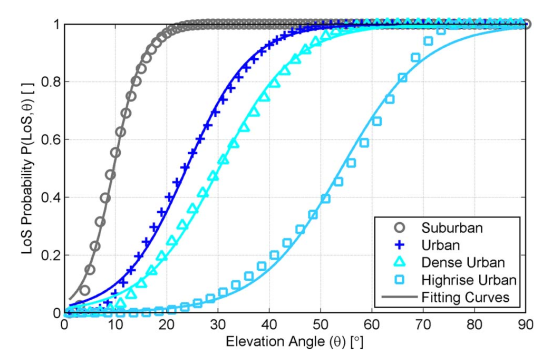
\includegraphics[width=5cm, height=3cm]{Figures/Figure2.png}
    \caption{The calculated LoS probabilities, with their related S-curve
fitting for different urban environments.}
    \label{fig:2}
\end{figure}
        
        \item We can notice that the trend can be closely approximated to a simple   modified Sigmoid function (S-curve) of the following form:
        \begin{align}
            P(LoS, \theta) = \frac{1}{ 1 + aexp (- b\left[\theta -  a\right])}
            \label{eqn:5}
        \end{align}
        where a and b are called here the S-curve parameters.
    \end{enumerate}
    % This approximation significantly ease the calculation of the LoS probability,

\end{frame}
\begin{frame}{}

\begin{enumerate}
    \item To generalize the solution we have linked the S-curve parameters a and b directly to the environment variables $\alpha, \beta$ and $\gamma$. This linking was performed using two variables surface fitting 
where 
\begin{enumerate}
    \item $(\alpha \times \beta)$ is assumed as the first variable
\item $(\gamma)$ as the second. 
\end{enumerate}
    \item The surface equation yields a two-variables polynomial having the following form:
    \begin{align}
        z = \sum_{j=0}^{3}  \sum_{i=0}^{3-j} C_{ij}(\alpha \beta)^i \gamma^j
        \label{eqn:6}
    \end{align}
    where 
    \begin{enumerate}
        \item z represents the fitting parameter a or b
        \item $C_{ij}$ are the polynomial coefficients
    \end{enumerate}


\end{enumerate}

    
\end{frame}
\begin{frame}{}
\begin{enumerate}
    \item To analyze the effect of the LAP’s altitude on the provided service, firstly we define the service threshold in terms of the maximum allowable pathloss $PL_{max}$.
    \item If the total pathloss between the LAP and a receiver exceeds this threshold then the link is deemed as failed.
    \item For ground receivers, this threshold translates into a coverage disk (zone) of radius R, since all receivers within this disk have a pathloss that is less than or equal $PL_{max}$
     \begin{figure}
    \centering
    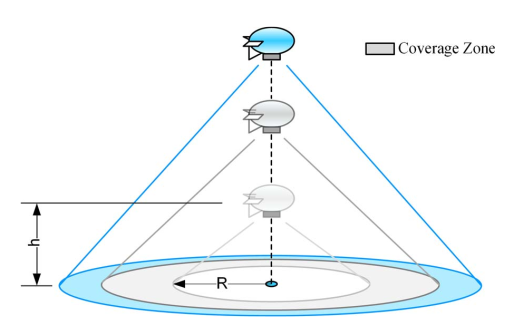
\includegraphics[width=5cm, height=3cm]{Figures/Figure3.png}
    \caption{The coverage zone by a low altitude platform.}
    \label{fig:3}
\end{figure}
    
\end{enumerate}
    
\end{frame}


\begin{frame}{}
    \begin{enumerate}
        \item Mathematically, the cell radius of the coverage zone can be written as:
        \begin{align}
            R = r|_{\Lambda = PL_{max}}
            \label{eqn:7}
        \end{align}
        \item Optimization problem is to find the best altitude that will maximize R.
        \begin{block}{Relation between the LAP altitude h and the cell radius R }
        By rewriting Equation (\ref{eqn:1}) we have: 
        \begin{align}
            PL_{LoS} &= 20 \text{ log } d + 20 \text{ log } f + 20\text{ log }(\frac{4 \pi}{c}) +   \eta_{LoS} 
            \label{eqn:8}\\
PL_{NLoS} &= \underbrace{20 \text{ log } d + 20 \text{ log } f + 20 \text{ log }(\frac{4 \pi}{c})}_\text{FSPL} +   \underbrace{\eta_{NLoS}}_\text{$\eta_\xi$}
\label{eqn:9}
        \end{align}where \begin{enumerate}
        \item The FSPL is according to Friis equation with
the assumption of isotropic transmitter and receiver antennas.
            \item $d = \sqrt{h^2 + r^2}$ , is the distance between the LAP and a receiver at circle of radius r
            \item f is the system frequency.
        \end{enumerate}
 
        \end{block}
    \end{enumerate}
\end{frame}

\begin{frame}{}
   \begin{enumerate}
       \item By solving equations (\ref{eqn:3}), (\ref{eqn:5}), (\ref{eqn:7}), (\ref{eqn:8}), (\ref{eqn:9})  we get 
       \begin{align}
           PL_{max} = \frac{A}{1+a exp\left(-b\left[ arctan(\frac{h}{R} - a\right] \right)} + 10 log(h^2 + R^2) + B
           \label{eqn:10}
       \end{align}
       where \begin{align*}
               A &= \eta_{LoS} - \eta_{NLoS} \\
               B &= 20log f + 20 log(\frac{4 \pi}{c}) +   \eta_{NLoS}
           \end{align*}
           \item In order to obtain the optimum point of the LAP altitude $h_{OPT}$ that yields the best coverage, we need to search for the value of h that satisfies the equation of the critical point:
           \begin{align}
               \frac{\partial R}{\partial h} = 0
           \end{align}
     
   \end{enumerate}
\end{frame}
\begin{frame}{}
\begin{columns}
\begin{column}{0.5\textwidth}
    \begin{figure}
    \centering
    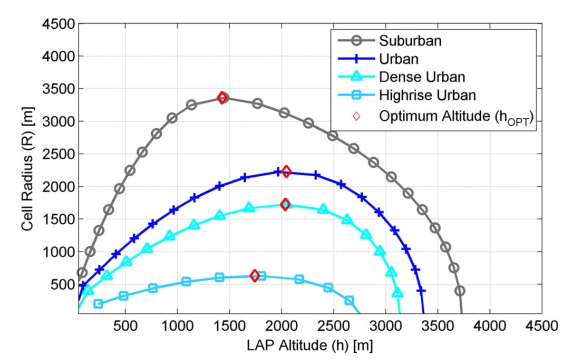
\includegraphics[width=5.67cm, height=3.64cm]{Figures/Figure4.png}
    \caption{Cell radius vs. LAP altitude curve for four different urban environments.}
    \label{fig:4}
\end{figure}
This shows that the optimum altitude of a LAP is strongly dependent on the specific urban environment condition.

\end{column}
\begin{column}{0.5\textwidth}  %%<--- here
    \begin{figure}
    \centering
    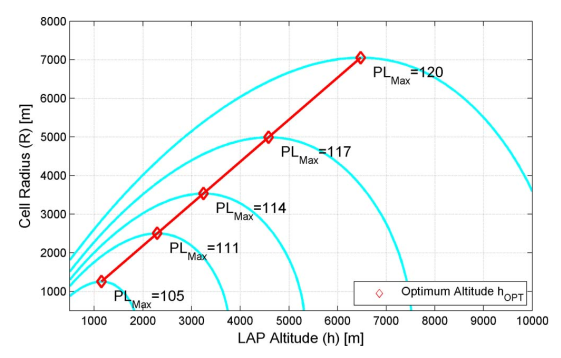
\includegraphics[width=5.61cm, height=3.58cm]{Figures/Figure5.png}
    \caption{Cell radius vs. LAP altitude curve for different maximum pathloss, in an urban environment.}
    \label{fig:5}
\end{figure}
We can notice that there is a certain elevation angle that always satisfies a constant ratio of $\frac{h_{opt}}{R}$, we call it here the optimum elevation angle or $\theta_{OPT} = arctan(\frac{h_{OPT}}{R})$
\end{column}
\end{columns}

\end{frame}

\begin{frame}{}
\begin{block}{Optimum Elevation angle}
On rewriting the expression in (\ref{eqn:10}) in terms of $\theta$ and $R$ as the following:

\begin{align}
    PL_{max} = \frac{A}{1 + a\text{ exp}(-b[\theta-a])} + 20\text{ log}(R\text{ sec}\theta) + B
\end{align}
The optimum point can then be found by solving the equation
$\frac{\partial R}{\partial \theta} = 0$, which yields the following:
\begin{align}
    \frac{\pi}{9\text{ ln}(10)}\text{ tan}(\theta_{OPT}) + \frac{abA \text{ exp}(-b[\theta_{OPT}-a])}{[a\text{ exp}(-b[\theta_{OPT}-a])+1]^2} = 0
     \label{eqn:13}
\end{align}
\end{block}
\begin{block}{Observation}
\begin{enumerate}
    \item  $\theta_{OPT}$ is independent of the maximum allowed pathloss
    \item It is also unique for a certain set of parameters ($a, b, A$)
\end{enumerate}

\end{block}
   
\end{frame}
\section{Conclusion}
\begin{frame}{Conclusion}
    
    \begin{enumerate}
        
% \item $PL_{max}$ depends on the sensitivity of the receiver, communication technology,and the target quality of service
% \item For large values of $PL_{max}$ the optimum altitude may exceed the earth’s atmosphere which is not a practically viable solution.
% \item So, the optimum altitude for the LAP can be the found by imposing a constraint on h in our proposed model.

\item We understood how Low-altitude aerial platforms (LAPs) have recently
gained significant popularity as key enablers for rapid deployable
relief networks where coverage is provided by onboard radio
heads.
\item We learnt a method for  optimizing the altitude of such platforms
to provide maximum radio coverage on the ground. 
\item Our analysis shows that the optimal altitude is a function of the maximum allowed pathloss and of the statistical parameters of the urban
environment,
    \end{enumerate}
    
\end{frame}
\end{document}
